%  \documentclass[DIV=12, a4]{scrartcl}
%\documentclass[12pt, a5]{scrartcl}
\documentclass[a4]{scrartcl}

\usepackage[
fancytheorems, 
noindent, 
%spacingfix, 
%noheader
]{adam}

\usepackage{tikz}
\usepackage{enumitem}

% \usepackage{subfig}

% \setcounter{section}{-1}

\title{Vectors and Matirces}
% \subtitle{Adam Kelly}
\author{Adam Kelly, Lectured by Dr. J. Evans}
\date{Michaelmas 2020}

\begin{document}

\maketitle

\begin{abstract}
	This document is an account of the Cambridge Mathematical Tripos course `Vectors and Matrics', lectured by Dr. Jonathan Evans in Michaelmas 2020.
	This is a work in progress, and is likely to to contain errors, which you may assume to be my own.
	% This document is a rather brief summary of the first three chapters of H. S. M. Coxeter and S. L. Greitzer's `Geometry Revisited'.
	% In no ways is this fleshed out, and in most cases just contains the important results and diagrams.
	% Specifically, it's purpose is to be somewhat of a reference which one can consult whilst attempting olympiad geometry problems.
\end{abstract}

\tableofcontents

\clearpage

\section{Introduction}

Vectors and Matrices covers topics in both algebra and geometry, and the way in which they relate to one another. The course uses approaches that are quite varied in their nature (can be abstract or more concrete, conceptual or more computational, and so on). You will need to be able to fluently switch between these approaches.

The course assumes that you are vaguely familiar with Euclidean and coordinate geometry, along with the idea of geometrical transformations.

\subsection{Course Structure}

This course is divided into a number of chapters.

\begin{enumerate}
	\item \emph{Complex Numbers}

	This chapter takes the point of view of thinking of points in the plane as pairs of real numbers, and defining `multiplication' on it to turn it into the complex numbers.

	\item \emph{Vectors in Three Dimensions}
	
	Here, we will recap on the relationship between three dimensional vectors and some of theire geometrical applications, and we will discuss things like the dot and cross product. Towards teh end of that discussion, we will introduce the `index notation', a powerful and helpful notation for dealing with vectors. We will also introduce the `summation convention', which is also incredibly useful.

	\item \emph{Vectors in a General Setting}
	
	This chapter will discuss what vectors are in general, and different ways of looking at them. We will be particularly concerned with vectors in $\mathbb{R}^n$ and $\mathbb{C}^n$, that is, vectors who's entries are in $\mathbb{R}$ and $\mathbb{C}$ respectively.

	\item \emph{Matrices and Linear Maps}
	
	Picking up on the idea of generalizing vectors, this chapter will consider the idea of a `linear map', an abstraction of matrices. 

	\item \emph{Determinants and Inverses}
	
	This chapter will detail how to define and compute determinants of general $n \times n$ matrices. This will take two points of view, in that we need to be able to compute them but we also must understand what they mean. The relation between determinants and finding inverses of matrices will also be considered.

	\item \emph{Eigenvalues and Eigenvectors}
	
	This chapter also involves both geometry and algebra. The core question of this chapter is: given a linear map or matrix, what does it act on in a very straightforward way?

	\item \emph{Changing Basis, Canonical Forms and Symmetries}
	
	In this final chapter, we will consider a set of far reaching results by trying to describing an arbitrary linear map. These ideas are far reaching, and immensely useful.
\end{enumerate}

\clearpage

\section{Complex Numbers}

\subsection{Definitions}

We construct the complex numbers $\mathbb{C}$ from the real numbers $\mathbb{R}$ by adjoining an element $i$ with $i^2 = -1$.
Any complex number $z \in \mathbb{C}$ has the form (by definition)
$$
z = x + iy,
$$
with $x, y, \in \mathbb{R}$. $x = \operatorname{Re}(z)$ is called the \vocab{real part}, and $y = \operatorname{Im}(z)$ is called the \vocab{imaginary part}.

With this definition of complex numbers, we can define how arithmetic works with them.

\begin{definition}[Arithmetic on Complex Numbers]
	For $z_1 = x_1 + i y_1$ and $z_2 = x_2 + i y_2$, we define
\begin{enumerate}[label=(\roman*)]
	\item \emph{Addition}. $z_1 + z_2 = (x_1 + x_2) + i(y_1 + y_2)$.
	\item \emph{Multiplication}. $z_1 z_2 = (x_1 + i y_1)(x_2 + i y_2) = (x_1 x_2 - y_1 y_2) + i(x_1 y_2 + x_2 y_1)$.
	\item \emph{Complex conjugation}. $\overline{z} = z^* = x - iy$.
	\item \emph{Modulus}. $r = |z|$ is a non-negative real given by $r^2 = |z|^2 = z \overline{z} = x^2 + y^2$.
	\item \emph{Argument}. For nonzero $z$, $\theta = \operatorname{arg}(z)$ is a real defined\footnote{$\operatorname{arg}(z)$ is determined modulo $2\pi$, which follows from $\tan \theta = x/y$.} such that $z = r(\cos \theta + i \sin \theta)$. This is the \vocab{polar form} of $z$.
	
	With this we have that
	$$
	\cos \theta=\frac{x}{\left(x^{2}+y^{2}\right)^{1 / 2}} \quad \quad \sin \theta=\frac{n}{\left(x^{2}+y^{2}\right)^{1 / 2}} \quad \implies  \quad \tan \theta=\frac{y}{x}.
	$$

	In order for $\theta$ to be unique, we can restrict the range of $\theta$. For example, if $-\pi < \theta \leq \pi$, we call this the \vocab{principle value}. However other choices of range are equally valid.
\end{enumerate}
\end{definition}

\begin{proposition}[Properties of Complex Conjugation]
	We have
	\begin{enumerate}[label=(\roman*)]
		\item $\operatorname{Re}(z) = \frac{1}{2}(z + \overline{z})$.
		\item $\operatorname{Im}(z) = \frac{1}{2i}(z - \overline{z})$.
		\item $\overline{(\overline{z})} = z$.
		\item $\overline{z_1 + z_2} = \overline{z_1} + \overline{z_2}$.
		\item $\overline{z_1 z_2} = \overline{z_1} \overline{z_2}$.
	\end{enumerate}
\end{proposition}
\begin{proof}[Proof Sketch]
	A direct check from the definitions.
\end{proof}


\begin{definition}[The Argand Diagram/Complex Plane]
	Plot $\operatorname{Re}(z)$ and $\operatorname{Im}(z)$ on orthogonal axes, then $r = |z|$ and $\arg(z) = \theta$ are the length and angle as shown.
	\begin{center}
		

\tikzset{every picture/.style={line width=0.75pt}} %set default line width to 0.75pt        

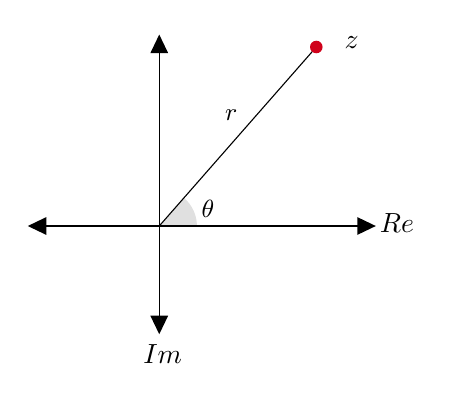
\begin{tikzpicture}[x=0.75pt,y=0.75pt,yscale=-1,xscale=1]
%uncomment if require: \path (0,300); %set diagram left start at 0, and has height of 300

%Shape: Pie [id:dp2413182761278425] 
\draw  [draw opacity=0][fill={rgb, 255:red, 224; green, 224; blue, 224 }  ,fill opacity=1 ] (182.32,96.76) .. controls (186.1,100.05) and (188.48,104.86) .. (188.49,110.23) -- (170.34,110.24) -- cycle ;
%Straight Lines [id:da39150586947897015] 
\draw    (246,24) -- (170.34,110.24) ;
%Straight Lines [id:da07162620321201185] 
\draw    (170.34,159.39) -- (170.34,21) ;
\draw [shift={(170.34,18)}, rotate = 450] [fill={rgb, 255:red, 0; green, 0; blue, 0 }  ][line width=0.08]  [draw opacity=0] (8.93,-4.29) -- (0,0) -- (8.93,4.29) -- cycle    ;
\draw [shift={(170.34,162.39)}, rotate = 270] [fill={rgb, 255:red, 0; green, 0; blue, 0 }  ][line width=0.08]  [draw opacity=0] (8.93,-4.29) -- (0,0) -- (8.93,4.29) -- cycle    ;
%Straight Lines [id:da3144480185294898] 
\draw    (271.68,110.24) -- (110,110.24) ;
\draw [shift={(107,110.24)}, rotate = 360] [fill={rgb, 255:red, 0; green, 0; blue, 0 }  ][line width=0.08]  [draw opacity=0] (8.93,-4.29) -- (0,0) -- (8.93,4.29) -- cycle    ;
\draw [shift={(274.68,110.24)}, rotate = 180] [fill={rgb, 255:red, 0; green, 0; blue, 0 }  ][line width=0.08]  [draw opacity=0] (8.93,-4.29) -- (0,0) -- (8.93,4.29) -- cycle    ;
%Shape: Ellipse [id:dp8293273168033899] 
\draw  [draw opacity=0][fill={rgb, 255:red, 208; green, 2; blue, 27 }  ,fill opacity=1 ] (242.98,24) .. controls (242.98,22.33) and (244.33,20.98) .. (246,20.98) .. controls (247.67,20.98) and (249.02,22.33) .. (249.02,24) .. controls (249.02,25.67) and (247.67,27.02) .. (246,27.02) .. controls (244.33,27.02) and (242.98,25.67) .. (242.98,24) -- cycle ;

% Text Node
\draw (284.89,108.73) node    {$\operatorname{Re}$};
% Text Node
\draw (172,172) node    {$\operatorname{Im}$};
% Text Node
\draw (263,22) node    {$z$};
% Text Node
\draw (193.78,101.93) node  [font=\small]  {$\theta $};
% Text Node
\draw (205,57) node  [font=\small]  {$r$};


\end{tikzpicture}
	\end{center}
\end{definition}

\begin{example}
	For $z = -1 + i \sqrt{3}$, we have $|z| = 2$ and $\arg(z) = \frac{2 \pi}{3} + 2n \pi$ for $n \in \mathbb{Z}$. This is shown on the complex plane below.

	\begin{center}
		

\tikzset{every picture/.style={line width=0.75pt}} %set default line width to 0.75pt        

\begin{tikzpicture}[x=0.75pt,y=0.75pt,yscale=-1,xscale=1]
%uncomment if require: \path (0,300); %set diagram left start at 0, and has height of 300

%Shape: Pie [id:dp2413182761278425] 
\draw  [draw opacity=0][fill={rgb, 255:red, 224; green, 224; blue, 224 }  ,fill opacity=1 ] (191.75,153.57) .. controls (195.34,151.46) and (199.53,150.25) .. (204,150.25) .. controls (217.25,150.25) and (227.99,160.88) .. (228,173.99) -- (204,174) -- cycle ;
%Straight Lines [id:da39150586947897015] 
\draw    (142,70) -- (204,174) ;
%Straight Lines [id:da07162620321201185] 
\draw    (204,243) -- (204,21) ;
\draw [shift={(204,18)}, rotate = 450] [fill={rgb, 255:red, 0; green, 0; blue, 0 }  ][line width=0.08]  [draw opacity=0] (8.93,-4.29) -- (0,0) -- (8.93,4.29) -- cycle    ;
\draw [shift={(204,246)}, rotate = 270] [fill={rgb, 255:red, 0; green, 0; blue, 0 }  ][line width=0.08]  [draw opacity=0] (8.93,-4.29) -- (0,0) -- (8.93,4.29) -- cycle    ;
%Straight Lines [id:da3144480185294898] 
\draw    (339,174) -- (69,174) ;
\draw [shift={(66,174)}, rotate = 360] [fill={rgb, 255:red, 0; green, 0; blue, 0 }  ][line width=0.08]  [draw opacity=0] (8.93,-4.29) -- (0,0) -- (8.93,4.29) -- cycle    ;
\draw [shift={(342,174)}, rotate = 180] [fill={rgb, 255:red, 0; green, 0; blue, 0 }  ][line width=0.08]  [draw opacity=0] (8.93,-4.29) -- (0,0) -- (8.93,4.29) -- cycle    ;
%Shape: Ellipse [id:dp8293273168033899] 
\draw  [draw opacity=0][fill={rgb, 255:red, 208; green, 2; blue, 27 }  ,fill opacity=1 ] (138,70) .. controls (138,67.79) and (139.79,66) .. (142,66) .. controls (144.21,66) and (146,67.79) .. (146,70) .. controls (146,72.21) and (144.21,74) .. (142,74) .. controls (139.79,74) and (138,72.21) .. (138,70) -- cycle ;

% Text Node
\draw (355.5,172) node    {$\operatorname{Re}$};
% Text Node
\draw (206,254) node    {$\operatorname{Im}$};
% Text Node
\draw (108.5,47) node    {$-1+i\sqrt{3}$};
% Text Node
\draw (140,128) node  [font=\small]  {$|z|=2$};
% Text Node
\draw (257,140) node  [font=\small]  {$\operatorname{Arg}( z) =\frac{2\pi }{3}$};


\end{tikzpicture}
	\end{center}

	Note that $\tan \theta = - \sqrt{3}$, so $\theta = \frac{2 \pi}{3} + 2n \pi$, or $\theta = -\frac{\pi}{3} + 2n \pi$, which is $\arg(-z)$. This is notable because it is common to write $\arg(z) = \arctan(y/x)$, but that is not quite correct.
\end{example}


\subsection{Basic Properties of Complex Numbers}

In this section, we will consider the consequences of the definitions given in the previous section.
Let us begin by defining the notion of a field.

\begin{definition}
	A \vocab{field} is a thing yeah.
\end{definition}

\begin{proposition}
	$\mathbb{C}$ with addition and multiplication is a field.
\end{proposition}
\begin{proof}
	Fill in details here.
\end{proof}

The next consequence is the `Fundamental Theorem of Algebra'.
This is something that's important to know about, but we will not prove it.

\begin{theorem}[Fundamental Theorem of Alegbra]
	A polynomial $p(z)$ of degree $n$ with coefficients in $\mathbb{C}$ can be written as a product of $n$ linear factors. That is, if we have a polynomial
	$$
	p(z) = c_n z^n + c_{n - 1} z^{n - 1} + \cdots + c_1 z + c_0
	$$
	with $c_i \in \mathbb{C}$ and $c_n \neq 0$, then we can write
	$$
	p(z) = (z - \alpha_1) (z - \alpha_2) \cdots (z - \alpha_n),
	$$ 
	for some $\alpha_i \in \mathbb{C}$ not necissarily distinct.
\end{theorem}
\begin{proof}[Proof Omitted]
	See the IB course `Complex Methods/Analysis'.
\end{proof}


% \begin{proposition}
% 	$\mathbb{C}$ is an abelian group under addition, and $\mathbb{C}\backslash\{0\}$ is an abelian group under multiplication.
% \end{proposition}
% \begin{proof}
% 	We note that addition and multiplication on complex numbers is both associative and commutative.
% 	For the group $(\mathbb{C}, +)$, we have the identity $0 + 0i$ and for $z = x + iy \in \mathbb{C}$, the inverse of $z$ is $-z$.  For the group $(\mathbb{C}\backslash\{0\}, \times)$, we have the identity $1 + i0$, and for nonzero $z = x + iy$, we have $z^{-1} = \frac{x}{x^2 + y^2} + i \frac{y}{x^2 + y^2}$, thus they are both abelian groups.
% \end{proof}



\end{document}
